% ---------------------------------------------------------------------
% This document compiles with pdflatex and is made with Koma-Script. 
%
% The Template is based on the template of Michael
% von Riegen, riegen@informatik.uni-hamburg.de, and
% modified at some points
% ---------------------------------------------------------------------
\documentclass[11pt,DIV=15,BCOR=20mm,bibliography=totoc, listof=totoc]{scrbook}

% Import of packages and options that refer to the whole document can be found in myPreamble.sty
\usepackage{myPreamble}
\usepackage{svg}
\usepackage{float}
\usepackage{listings}
\usepackage{multirow}
\usepackage{hyperref}
\usepackage{url}
\newacronym{udp}{UDP}{User Datagram Protocol}
\newacronym{tcp}{TCP}{Transmission Control Protocol}
\newacronym{des}{DES}{Discrete-Event Simulation}
\newacronym{rpc}{RPC}{Remote Procedure Call}
\newacronym{protobuf}{Protobuf}{Protocol Buffer}
\newacronym{nat}{NAT}{Network Address Translation}


% useful if writing everything in one chapter
%has no affection on input-commands
% \includeonly{kapitel1}

\begin{document}

	% titlepage
	\begin{titlepage}
%TODO personalize titlepage
	% Suppress error "destination with the same identifier"
  \setcounter{page}{-1}
    \definecolor{uhhred}{cmyk}{0,100,100,0}
    \renewcommand{\familydefault}{\sfdefault}
\frontmatter
\newgeometry{centering,left=3.7cm,right=2cm,top=2cm,bottom=2cm}
	% Titlepage
	\begin{figure}[h]
		\begin{minipage}[b]{62mm}
			
\includegraphics[width=62mm]{images/unilogo.png}
		\end{minipage}
		\hspace{4cm}
		%\begin{minipage}[b]{59mm}
		%	\includegraphics[width=59mm]{images/minlogo}
		%\end{minipage}
	\end{figure}

	\vfill
	\Large
	
\begin{center}
{\usefont{T1}{cmss}{bx}{n}
	%{\color{uhhred}\LARGE\textbf{\so{MASTERARBEIT}}}
	{\color{uhhred}\LARGE\textbf{\so{BACHELORARBEIT}}}
	\vspace*{1.5cm}
	
	{\LARGE \textbf{Fast and Reliable Scheduling of Discrete-event Simulation Runs in Heterogeneous Edge Computing Environments}}}
	\vspace*{1.75cm}\\
	vorgelegt von
	\vspace*{0.4cm}\\
	\LARGE Patrick Zierahn
\end{center}
\vspace*{3.7cm}

\noindent
MIN-Fakultät \vspace*{0.2cm} \\
Fachbereich Informatik \vspace*{0.2cm} \\
Arbeitsbereich Verteilte Betriebssysteme \vspace*{0.2cm} \\
Studiengang: B.Sc. Informatik \vspace*{0.2cm} \\ 
Matrikelnummer: 7065799 \vspace*{0.5cm} \\
Abgabedatum: 21.10.2021 \vspace*{0.2cm} \\ 
Erstgutachter: Prof. Dr. Janick Edinger \vspace*{0.2cm} \\
Zweitgutachter: Arne Koors
\end{titlepage}


	\cleardoubleemptypage
	\chapter*{Abstract}
Edge Computing can be a useful tool to speed up computationally intensive discrete event simulations. Most previous approaches for offloading OMNeT++ simulations are deprecated and cannot communicate peer-to-peer across various networks. This work presents a framework to offload OMNeT++ simulations to an edge computing peer-to-peer network using Go, gRPC, and UDP-Holepunching techniques. The distribution of simulation-runs by this work shows promising results in real-world trials. The execution time was reduced significantly by employing multiple devices across several networks.


	% roman page numbering
	%\frontmatter
	
	% lists (table of contents, list of figures, tables, abbreviations)
	\tableofcontents
	\listoffigures
	\listoftables
	\printglossary
	\printglossary[title=List of Abbreviations,type=\acronymtype]	
	
	% arabic page numbering
	\mainmatter
	
	\chapter{Introduction}

\section{Motivation}
\label{Motivation}

Besides experiments and theoretical analytic methods, simulations are considered to be one epistemic source of new knowledge \cite{standford:simulations}. Simulations are used to explain how we should expect some system in the real world to behave under a particular set of circumstances \cite{ingalls2011introduction}.

Extensive simulations like climate simulations or physical simulations \cite{10.1093/mnras/stt1403} require considerable resources to produce results in a reasonable time. Today many simulations are run on high-performance computers \cite{spataro2017high}. The cost of such devices is immensely high. The use of distributed edge computing might offer an alternative \cite{shi2016edge}.

Simulations are particularly interesting in edge computing research. The paper "Decentralized Low-Latency Task Scheduling for Ad-Hoc Computing" \cite{edinger2021decentralized} is one example where simulations play an important role. Simulating and modeling these systems offers a valid alternative to costly real world experiments.

Running simulations can be a time-consuming activity. For running simulations in practice, researchers often need to rent Cloud CPU-Clusters. These resources can be ex- pensive and involve bureaucratic challenges. CPU-Clusters also need lead time to be set up, which prevents spontaneous use. The addition of idle devices like laptops or Raspberry Pis is also currently not realizable. Employing idle edge resources across many networks could offer an attractive alternative to the described laborious process.


\section{Goals of the Thesis}
\label{Goals-of-the-Thesis}

Accelerating more complex simulations is increasingly crucial for scientific progress. This thesis aims to enable the spontaneous use of local and distributed edge devices for discrete event simulations. Through distribution and parallelization, the simulation process should accelerate.

This work aims to build a tool that can distribute discrete event simulations written with OMNeT++ to multiple end-user instances, execute it there and transfer the results back afterward. In the end, the source folder should contain the results like they were run locally. By distributing and parallelizing the simulation should thereby accelerate the execution compared to local ones.

The tool should be able to connect to providers in the local network and other networks. Consumers and providers communicate directly over peer-to-peer connections to ensure maximal scalability. If the peer-to-peer connection fails, providers and consumers can use relay services.

Users should be able to conveniently deploy the software in the form of Docker containers. The Docker container should include everything needed to participate in the resource sharing network to make it easy to add resources spontaneously.

\section{Structure of this work}
The fundamentals explain basic terminology and technologies used throughout this work. The related work chapter scrutinises related approaches for simulation distribution. The design Chapter exhibits the proposed distribution and parallelizing mechanisms. The implementation chapter lines out the technical realization of the in the design chapter proposed mechanisms. Real world experiment results are assessed in the evaluation chapter. The conclusion summarizes this work and the further research Section describes further research areas.

	\chapter{Fundamentals}

The following Chapter will outline the basics concepts of distributed computing, discrete event simulations in conjunction with OMNeT++, remote procedure calls with gRPC, and the QUIC protocol.

\section{Distributed Computing}

A distributed computer system consists of multiple software components located on multiple computers but runs as a single system. The computers that belong to distributed systems can be physically close together and connected by a local network, or they can be geographically distant and connected by a wide area network \cite{ibm:distributedcomputing}.

Grid computing is the use of widely distributed computer resources to reach a common goal. A computing grid can be thought of as a distributed system with non-interactive workloads that involve many files. Grid computing is distinguished from conventional high-performance computing systems such as cluster computing \cite{foster2008cloud}. In grid computers each node is set to perform a different task/application. In high-performance computing systems each computer code works on the same task/application. Grid computers also tend to be more heterogeneous and geographically dispersed (thus not physically coupled) compared to cluster computers \cite{wiki:Grid_computing}.

Edge computing is a paradigm in which substantial computing and storage resources are placed at the Internet’s edge in close proximity to mobile devices or sensors that generate and process data \cite{satyanarayanan2017emergence}. In the Cloud computing paradigm, most of the computations happen in a centralized cloud. The cloud computing paradigm may suffer longer latency, which impairs user experience \cite{shi2016edge}. 

\section{OMNeT++ Discrete Event Simulator}

A discrete-event simulation (DES) models a system as a discrete sequence of events in time. Each event occurs at a particular point in time and signals a change of state in the system \cite{wiki:des}. They are contrasted by continuous simulations which refers to a computer model of a physical system that continuously tracks system response according to a set of equations involving differential equations \cite{wiki:contsim}.

OMNeT++ is a discrete event network simulation framework. It provides infrastructure and tools for writing simulations. OMNeT++ can be installed with an integrated development environment (IDE) but it can also be run as a command line tool. It is used to simulate various problem domains for example modeling of wired and wireless communication networks, protocol modeling, and evaluating performance aspects of complex software systems. In general it is used for modeling and simulating any system that consists of discrete events. OMNeT++ simulations are composed of reusable modules that are commonly written in C++. Modules are generic parts and can be used across various projects \cite{oppSimulationManual5.6.1}.

The simulation needs to be compiled before execution. A makefile for the simulation can be created using the opp\_makemake command line tool installed with OMNeT++. Opp\_makemake can be configured to output either a simulation executable or a static or dynamic library. The simulation can be compiled afterwards by calling make.

OMNeT++ uses NED files to define components and to assemble them into larger units like networks. INI files tell the simulation program which network should be simulated (NED files may contain several networks). They are also used to pass parameters and parameter combinations to the model. Explicit seeds for the random number generators are specified the same way. OMNeT++ can be used for parameter studies, where a combination of different parameters is the subject of study. INI files specify these parameter combinations. Each INI file can have various parameter configurations. Each parameter combination belongs to one simulation run that can be executed concurrently \cite{omnetpp:tictoc}.

OMNeT++ simulations are composed out of reusable modules. Modulus are commonly written in C++. Hence they need to be compiled before the execution.

\begin{lstlisting}[caption=Example INI file]
[Config Tictoc7]
network = Tictoc7
# argument to exponential() is the mean; truncnormal() returns values from
# the normal distribution truncated to nonnegative values
Tictoc7.tic.delayTime = exponential(3s)
Tictoc7.toc.delayTime = truncnormal(3s,1s)

[Config Tictoc16]
network = Tictoc16
**.tic[1].hopCount.result-recording-modes = +histogram
**.tic[0..2].hopCount.result-recording-modes = -vector

[Config Tictoc17]
network = Tictoc17

[Config TicToc18]
network = TicToc18
sim-time-limit = 250h
**.tic[*].hopCount.result-recording-modes = +vector
*.numCentralNodes = ${N=100..200 step 4}
repeat = 3
\end{lstlisting}

The simulation can be run as an executable or as a library, to run it NED and INI files need to be passed to it. If the simulation is compiled as an executable, the executable will be called with "-n" to specify the NED paths and "-f" to pass the INI file paths. If the simulation was compiled as a library, the command is "opp\_run -l LIBRARY." The parameter "-u Cmdenv" denotes that the simulation is run from a command-line environment. This parameter prevents the attempt to start the OMNeT++ IDE. The parameter "-c" tells the simulation which configuration from the INI files should be executed.

Execute the simulation:
\begin{itemize}
  \item Run the simulation as an executable: "./tictoc -n . -f omnetpp.ini -u Cmdenv -c TicToc18"
  \item Run the simulation as a library: "opp\_run -l tictoc -n . -f omnetpp.ini -u Cmdenv -c TicToc18"
\end{itemize}

The simulation can output all configurations with the associated number of runs.
\begin{itemize}
  \item Extract configurations: "./tictoc -f omnetpp.ini -n . -a"
  \item Extract run numbers: "./tictoc -f omnetpp.ini -n . -c TicToc18 -q runnumbers"
  \item Execute a simulation run: "./tictoc -f omnetpp.ini -n . -c TicToc18 -r 123"
\end{itemize}

\section{gRPC}

In distributed computing, a remote procedure call (RPC) is when a computer program calls a procedure on another computer. The procedure is, as a result of this, called like a locally coded function. The programmer does not have to explicitly code the details of the remote interaction and can write the same code whether the procedure is local or remote. The caller is the client, and the executor is the server \cite{wiki:Remote_procedure_call}.

gRPC is a request-response message-passing system for remote procedure calls. gRPC is based around the idea of defining a service, specifying the methods that can be called remotely with their parameters and return types. The server implements this interface and runs a gRPC server to handle client calls. The client has a local object that provides the same methods as the server \cite{grpc:introduction}.

\begin{figure}[h]
  \centering
  \includesvg[width=250pt]{images/gRPC-Overview.svg}
  \caption{Overview of gRPC communication}
  \label{fig:grpcoverview}
\end{figure}

gRPC clients and servers can run and communicate with each other in a variety of environments. For example, gRPC can create a server in Java with clients written in Go, Python, or Ruby. Figure \ref{fig:grpcoverview} shows this.

gRPC uses Protocol Buffers as the Interface Definition Language (IDL) for describing both the service interface and the structure of the payload messages. Each message contains a series of name-value pairs called fields. Once the data structures are specified, the protocol buffer compiler protoc generates client- and server-side code in the preferred programming language.

gRPC lets you define four kinds of service method:
\begin{itemize}
    \item "Unary RPCs where the client sends a single request to the server and gets a single response back, just like a normal function call." \cite{grpc:concepts}
    \item "Server streaming RPCs where the client sends a request to the server and gets a stream to read a sequence of messages back. The client reads from the returned stream until there are no more messages." \cite{grpc:concepts}
    \item "Client streaming RPCs where the client writes a sequence of messages and sends them to the server, again using a provided stream. Once the client has finished writing the messages, it waits for the server to read them and return its response." \cite{grpc:concepts}
    \item "Bidirectional streaming RPCs where both sides send a sequence of messages using a read-write stream. The two streams operate independently, so clients and servers can read and write in whatever order they like: for example, the server could wait to receive all the client messages before writing its responses, or it could alternately read a message then write a message, or some other combination of reads and writes. The order of messages in each stream is preserved." \cite{grpc:concepts}
\end{itemize}

RPCs can convey metadata in the form of a list of key-value pairs, where the keys are strings, and the values are typically strings. gRPC allows clients to specify how long they want to wait for an RPC to complete before the RPC exits with a timeout error. The server can query to see if a particular RPC has a deadline. Either the client or the server can cancel an RPC at any time. A cancellation terminates the RPC immediately.

\section{Peer-to-Peer (P2P) Networks}

Network address translation (NAT) is a method for routing devices of mapping an IP address space into another. NAT is an essential tool in maintaining global address space in the face of IPv4 address exhaustion \cite{durand2011dual}. One IP address of a NAT gateway can be shared across an entire private network. There are various types of NATs, including Full Cone NATs, Restricted Cone NATs, Port Restricted Cone NATs, and Symmetric NATs. \cite{wei2008new}

Peer-to-Peer (P2P) networks work on the presumption that all nodes in the network are connectable. However, NAT boxes and firewalls prevent connections to many nodes on the Internet. For UDP-based protocols, the UDP hole-punching technique has been proposed to mitigate this problem. \cite{halkes2011udp}

\section{QUIC}

QUIC is an abbreviation for "Quick UDP Internet Connections." It is an encrypted, multiplexed, and low-latency transport protocol. One advantage of QUIC against TCP is that it is a user-space transport protocol that can be changed easier than kernel-based approaches like TCP. QUIC eliminates Protocol Entrenchments, Implementation Entrenchments, Handshake Delays, Head-of-line Blocking Delays. It also has mechanisms for Loss Recovery and NAT Rebinding. \cite{langley2017quic}


	\chapter{Related Work}

There have been several related efforts to use distribution across multiple devices to advance the simulation execution time. None of which considers using end-user devices and edge devices for simulation execution. Table \ref{tab:relatedworks} shows relevant features that are covert by the approaches.

\begin{table}[h]
\begin{center}
    \begin{tabular}{ | m{10em} | m{6em}| m{6em} | m{6em} | m{5em} | }
      \hline
      Project & Edge devices and end-user devices & Peer-to-peer network & Spontaneous resource usage & Deprecated \\ 
      \hline
      Deploying on AWS & No & No & No & No \\
      \hline
      Remote OMNeT++ & No & No & Yes & Yes \\
      \hline
      Grid based systems & No & No & Yes & Mostly \\
      \hline
    \end{tabular}
    \caption{\label{tab:relatedworks} Related works}
\end{center}
\end{table}


\section{Remote OMNeT++}
Remote OMNeT++ is a now-discontinued effort to run simulations on a remote host. It creates a simulation environment that provides the same functionality whether used locally or remotely. Clients are equipped with web-based software that gives them the tools to connect to hosts, manage models and run a simulation. Processing Hosts are usually high-performance computers. Data Warehouses are high storage capacity machines that store models and simulation results. The program is written in Java and uses remote procedure calls to convey instructions. It comes with a "robust authentication and administration mechanism in place" \cite{erdei2002networked}.

\section{AWS Deployment}
The OMNeT++ website offers instructions on how to deploy and distribute simulations in the AWS cloud. Docker containers contain an OMNeT++ environment and the python worker software that executes the simulation. Simulation-runs are queued in a Redis database and dequeued by workers. AWS ECS instances deploy the containers. Simulations are offloaded by a Python script that adds the simulation-runs and model source to the Redis job queue \cite{omentpp:AWS}. Figure \ref{fig:omnetppaws} shows the architecture.

\begin{figure}[h]
  \centering
  \includesvg[width=\textwidth]{images/omnetpp-aws.svg}
  \caption{OMNeT++ AWS Architecture}
  \label{fig:omnetppaws}
\end{figure}

\section{Grid Computing}

There are several other approaches that use grid computing.
\begin{itemize}
  \item Xgrid was a batch queueing system for Apple computers. It was intended to enable the ad hoc bundling of a group of Macs into a grid computing cluster. Seggelmann showed in this work how to exploit Xgrid installations for running OMNeT++ simulations \cite{seggelmann2009parallelizing}. The underlying Apple software that enabled the distribution of tasks over a network has been deprecated since OS X v10.8 \cite{wiki:xgrid}.
  
  \item The paper "Enabling OMNeT++-based Simulations on Grid Systems" describes how the gLite batch queuing system can be used to distribute OMNeT++ simulations \cite{kozlovszky2009enabling}. gLite has been fully retired since May 1, 2013 \cite{web:glite}.

  \item RSerPool (Reliable Server Pooling) is an IETF protocol for server pool management and access \cite{dreibholz2008reliable}. It offers load balancing and failure handling capabilities. The SimProcTC toolchain offers makefiles and scripts to offload OMNeT++ simulations to remote hosts \cite{dreibholz2008powerful}. SimProcTC uses the RSerPool implementation to find suitable resource providers. The simulations are uploaded with all executables to the host and extracted there. A control script executes simulation-runs and retrieves the results. Parallelism is achieved via using parallel make jobs.

\end{itemize}

	\chapter{Design}

The distribution process for discrete event simulations written with OMNeT++ can be described in the following phases:
\begin{enumerate}
    \item In the "Prepare for Distribution" phase, the simulation configurations will be sourced, and the simulation will be compressed.

    \item The "Retrieve Provider List" retrieves a list of providers that can be connected and enlisted for the offloading process.

    \item In the "Establish a Direct Connection" phase, a direct connection will be established to the providers.

    \item With the "Deploy the Simulation" phase, the providers will be prepared to execute the simulation. The source code will be uploaded and compiled.

    \item In the "Execute the Simulation" phase, the simulation-runs will be executed, and the results will be downloaded.
\end{enumerate}

\section{Entities}
Providers are entities that provide resources to the network. These resources include CPU power, RAM, storage, and network. Consumers can use these resources. The provider software should support heterogeneous devices like Raspberry Pis, Personal computers, and cloud computing instances. Hence, the distribution must be robust and reliable because providers can always drop the execution if the host system needs the resources.

Consumers are entities that like to offload OMNeT++ simulations. They distribute the simulation runs across providers to parallelize the execution.

The broker is a central node for consumers and providers to exchange connection information.

\section{Prepare for the Distribution}
Before the consumer can distribute the simulation to providers, some paths in the local files system are required. Firstly, the path to the OMNeT++ simulation source directory which should be dispersed. Second, the path to a configuration file that holds the following information.

\begin{itemize}
    \item Paths to NED and INI files.
    \item The OMNeT++ simulation configurations that should be run.
    \item Information about the compile process. For example, if the simulation should be compiled and used as a library. More complex simulations, that for example use the opp\_featuretool, require a build script. For simple projects a Makefile is created automatically.
    \item Paths to where to execute the simulation (basePath) and where the source code is located (sourcePath).
    \item Which files should be excluded from the simulation and distribution process. For example the .git directory.
    \item The path to the simulation executable or simulation library.
\end{itemize}

Afterward, the simulation source is compressed, and a unique simulation-id is generated. Next comes the connection phases to the providers.

\section{Retrieve a Provider List}

Before the consumer can connect to any provider, a list must be marshaled to hold all available providers. The consumer connects to the broker to acquire a list of available providers. The consumer then connects to the providers directly to reduce the traffic that would otherwise be sent through a central node. This is necessary to build an efficient and scalable network.

The broker sends a list with providers and their corresponding dial addresses to the consumer every time a provider joins or leaves. Providers register at the broker with their unique provider-id. After a provider has registered at the broker, the consumer gets an event with a list of all providers and their connection ids. After each event, the consumer tries to connect to the new providers directly. See graphic \ref{fig:sequence-connect} for a visual impression of this process.

\begin{figure}
  \centering
  \includesvg[width=400pt]{images/Sequence Connect.svg}
  \caption{Sequence diagram for fetching the provider list}
  \label{fig:sequence-connect}
\end{figure}

\section{Establish a Direct Connection}
\label{Establish-a-Direct-Connection}

There are three ways for providers and consumers to connect. The first is through discovery and connection in the local network. The second is using a peer-to-peer connection. The third is through a relay server which forwards all traffic if the peer-to-peer connection fails. An overview is depicted in Figure \ref{fig:connection-methods}.

The consumer will connect to the provider by dialing the provider-id. The broker enables the exchange of the connection information to establish peer-to-peer connections and offers relay services.

\begin{figure}[h]
  \centering
  \includesvg[width=400pt]{images/Top Down Connection.svg}
  \caption{Overview of connection methods}
  \label{fig:connection-methods}
\end{figure}

\subsection{Connect over the Local Network}
\label{Connect-over-the-Local-Network}
If consumers and providers are in the same network, they can connect directly to prevent unnecessary overhead. The consumer sends a UDP multicast broadcast with the dial-address as a payload to the local network. If the provider-id matches the dial address, providers in the local network will respond with a port number on which to connect. See graphic \ref{fig:Sequence-Stargate-Local}.

\begin{figure}[h]
  \centering
  \includesvg[width=400pt]{images/Sequence Stargate Local.svg}
  \caption{Sequence diagram for local stargate connection}
  \label{fig:Sequence-Stargate-Local}
\end{figure}

\subsection{Connect over Peer-to-Peer through NAT Traversal}
\label{Connect-over-Peer-to-Peer}

If the local peer discovery and connection process fail, a peer-to-peer connection will be tried. In peer-to-peer connections, both peers connect to each other's IP and port number directly. Establishing such a connection can be challenging because of interfering NATs and firewalls \cite{wei2008new}. TCP-Holepunching or UDP-Holepunching techniques can be used to establish a connection through a NAT. This thesis will focus on UDP-Holepunching techniques because they are simpler to establish.

Two steps are necessary to initiate a peer-to-peer connection over UDP. The first is the exchange of connection details, like IP addresses and port numbers. The second is the establishment of a direct connection. 

The broker will handle the exchange of IP addresses and port numbers. Figure \ref{fig:Sequence-Peer-Resolving} depicts the entire process.

\begin{figure}[h]
  \centering
  \includesvg[width=400pt]{images/Sequence Peer Resolving.svg}
  \caption{Sequence diagram of the peer resolving process}
  \label{fig:Sequence-Peer-Resolving}
\end{figure}

When peer-1 and peer-2 try to connect to one other, they have to send the same dedicated dial address to the broker. The broker will match those dial addresses and exchange the IPs and port numbers. 

In step one, Peer-1 sends the dial address to the broker. With this step, the broker stores the incoming IP address and port number together with the dial address. Step one will be repeated periodically to prevent the deprecation of connection data. This happens for example when the IP address changes.

The periodical repetition of step two is necessary to prevent the NAT gate from closing. The advantage is that the exchange does not have to occur immediately; a dialer can linger for some time.

Step three checks if the dial address is already registered. If this is the case the connection information like IP and port is exchanged in step four. The broker also decides which peer is peer-1 and which peer is peer-2.

After the connection information has been exchanged, a UDP connection between the peers will be established. Both peers need to actively send and receive messages simultaneously to punch a hole in NATs and firewalls. Figure ~\ref{fig:Sequence-NAT-Firewall} shows this.

\begin{figure}[h]
  \centering
  \includesvg[width=400pt]{images/Sequence NAT Firewall.svg}
  \caption{Example for NAT firewall}
  \label{fig:Sequence-NAT-Firewall}
\end{figure}

NAT firewalls will block packages from unknown destinations. If Peer-1 tries to send data to Peer-2 without Peer-2 having sent anything to Peer-1, the data will be lost. This is visible in Figure \ref{fig:Sequence-NAT-Firewall}. Because of this, both peers have to send a message to one another to open the firewall. Due to time discrepancies between the peers, the one peer is probably first. The UDP packages will be blocked by the firewall or ignored by the receiver. 

\begin{figure}[h]
  \centering
  \includesvg[width=400pt]{images/Sequence NAT Traversal.svg}
  \caption{Sequence diagram for NAT Traversal}
  \label{fig:Sequence-NAT-Traversal}
\end{figure}

Both peers exchange messages to verify that the connection is working correctly. Peer-1 sends a hello message to peer-2. Peer-2 then responds with an acknowledgment that the message was received back to peer-1. Peer-1 then sends an acknowledgment that the acknowledgment was received. This way, both peers sent and received data from another. If messages are lost or blocked by firewalls, the connection process will timeout and fail.

\subsection{Connect over a Relay Server}
\label{Connect-over-a-Relay-Server}

\begin{figure}[h]
  \centering
  \includesvg[width=400pt]{images/Sequence Relay Server.svg}
  \caption{Sequence diagram for relay connection}
  \label{fig:Sequence-Relay-Server}
\end{figure}

If the peer-to-peer connection fails, providers and consumers can use a relay server to establish a connection. The broker, as a result of this, forwards the entire traffic between provider and consumer.

Both peers connect to the broker over TCP. Afterward, both peers send the desired dial address to the broker. When the dial addresses can be matched, a success message is sent to both peers to confirm that the link was successful. After that, the same TCP connection is used to communicate between peers. See figure \ref{fig:Sequence-Relay-Server}.

\section{Deploy the Simulation}

After a successful connection, the deployment phase begins. In this phase, the provider is prepared to execute the simulation. The consumer creates a new session for the simulation on each provider. The simulation-id identifies a session and is generated to ensure less overhead when a consumer connects to a provider. They store for example if the simulation was uploaded and extracted. Sequence diagram \ref{fig:Sequence-Deploy-Detail} shows this process. Sessions also contain a deadline of how long the simulation is allowed to be stored and run on the provider. After a session is created, the simulation source will be uploaded to the provider and extracted to a directory with the simulation-id. 

\begin{figure}[h]
  \centering
  \includesvg[width=400pt]{images/Sequence Deploy Detail.svg}
  \caption{Sequence diagram for the deployment process with session details}
  \label{fig:Sequence-Deploy-Detail}
\end{figure}

Because the simulations are written in C++, they need to be compiled before they can be executed. The simulation should only be compiled once for each architecture and operating system. The provider that establishes a connection first is chosen to do this. After the simulation is compiled, only the binaries and executables are compressed and transferred back to the consumers. Subsequently, the consumer distributes the data to all other providers. The binaries are not exchanged between the providers directly because they can always join or leave. Graphic \ref{fig:Sequence-Deploy-Arch} shows this process in a simplified way (session updates and extract operations are not included for clarity reasons).

\begin{figure}[h]
  \centering
  \includesvg[width=400pt]{images/Sequence Deploy Arch.svg}
  \caption{Sequence diagram of the deployment process with different architectures}
  \label{fig:Sequence-Deploy-Arch}
\end{figure}

\section{Execute the Simulation}

After the simulation is deployed, the simulation run numbers will be extracted. The run numbers can be distributed across many devices, and a parallelization process can start. Each provider can run multiple simulation-runs simultaneously, and every consumer can run simulations on various providers. The blocking or overuse of resources can stall the simulation process. Hence an allocation process is essential. Providers assign consumers a number of jobs they are allowed to start (see figure \ref{fig:Sequence-Execute}). If a simulation is canceled, the provider needs to reassign allocated resources. Because the consumer requests resources from multiple providers, more jobs can be assigned than required to run the simulation, which results in a blocking of precious resources. When this happens, the consumer is obligated to return the overallocated resources.

\begin{figure}[h]
  \centering
  \includesvg[width=400pt]{images/Sequence Execute.svg}
  \caption{Sequence diagram of simulation allocation and execution process.}
  \label{fig:Sequence-Execute}
\end{figure}

With each allocation, the consumer can start a simulation run on the dedicated provider. Each simulation run can have a different execution time and write result files non deterministically within its project structure. If all runs are executed in parallel in the same directory, it is impossible to tell which process wrote what. To mitigate this, each process needs its own source directory. Copying the whole source directory can be taxing, to prevent this symlink links will be created for each file in the source directory. This procedure is called “Fake Copy” in this work. Within a fake copied directory, each simulation run can alter and write files. These files can be easily detected, compressed, stored, and transferred to the consumer without interfering with other simulation runs.

The consumer downloads and merges the results from the provider with the original simulation source directory. The simulation source directory will contain the results of the simulation like they were run by OMNeT++ locally.

	\chapter{Implementation}

This project is realized in Go. Go is an open-source programming language that makes it easy to build simple, reliable, and efficient software \cite{go:web}. Go brings many concurrency features like lightweight multiplexed threads, typed conduits named channels which allow goroutines to synchronize without explicit locks or condition variables \cite{go:tour}. Go's sync package provides Mutexes, Conds, Once, and more. It also comes with cross-platform support and rich cross compilers.

The source code will be structured into the following packages: 
\begin{itemize}
  \item Broker contains everything for the broker service.
  
  \item Cmd contains all program entry points and main functions for the different opp\_edge tools.
  
  \item Gconfig contains configuration definitions and default values used by various packages. It parses command-line arguments to change the following values dynamically: broker address and port number, the Stargate port number, worker name, and how many jobs start. It also provides the OS-specific paths to the cache and configuration directory.
  
    \item Omnetpp contains command-line wrappers for OMNeT++. This package can clean and compile the simulation, extract simulation configurations and run numbers. It also executes simulation runs.
    
    \item Proto contains the Protobuf and gRPC service definition files for the Broker, Storage and the Provider. It also includes the generated Go code from the definition files.

    \item Provider contains the gRPC Provider service implementation, a resource allocator, connection listeners, and the implementation for running the simulation, compressing results.

    \item Simple contains generic helper functions.
    
    \item Stargate establishes connections over the local network, peer-to-peer, or a relay server. It also handles the NAT-traversal process.
    
    \item Mimic contains tools that turn UDP connections into QUIC connections. It also includes utils that use QUIC connections to mimic TCP connections. These tools are needed to establish gRPC connections over UDP and QUIC.
    
    \item Stargrpc is the "gRPC over stargate" package. It employs Stargate and Mimic to create gRPC connections and servers.
    
    \item Storage transfers files between two devices. It holds helper functionality to simplify the transfer of large files.
\end{itemize}

\section{Simple}
The simple package contains generic helper functions used across many packages.

The FakeCopy function will create symlinks in the target directory, which point to all files in the source directory. The function will recreate every directory in the source in the target. Think of this as a copy function for directories that creates a symlink instead of an actual copy for files.

Simple also contains functionality to handle the extraction and compression of files. TarGzFiles tars and compresses files. Symlinks are handled correctly, an implementation for other special files like fifos is currently missing. TarGz tars and compresses all files in a directory. Files can be excluded by defining regexes that will be matched against file paths. ExtractTarGz extracts a tar gzip archive to the desired destination. The input is the compressed archive as a byte array.

Simple provides the functionality to identify files that changed in a directory. ListDirChecksum returns a list of all files in the given directory with its blake2b checksum. The blake2b is used because it is faster than MD5, SHA-1, SHA-2, and SHA-3. DirDiff compares the checksums of two file lists with one another. The files that do not match will be returned. The FilesChangeDetector is a struct that detects and bundles modified files that were changed. To do this, it creates a list of files and their checksums at the beginning. The ZipChanges function is called after changes in the directory occur. The function creates a new file list with checksums and compares these to the original list. Only the changed files will then be compressed and returned.

\section{Stargate}
The Stargate module establishes direct UDP and TCP connections between providers and consumers over the local network, peer-to-peer, or a relay server. Before the connection process can start both peers need to know where the server for the exchange of connection information is located. SetConfig sets the address and port number of this server.

The Stargate server starts TCP and UDP listeners on the same port number. The UDP listener is used to broker peer-to-peer connections. The TCP listener is used to broker relay connections.

To connect two peers it is necessary that both have the same dial address in the form of a string. This string is typically the provider-id. DialLocal broadcasts the dialAddr to the local network. It returns a TCP address on which to connect to the peer. BroadcastTCP is the counterpart to this process, it listens for multicast broadcasts and responds with a port on which to connect if the dialAddr matches.

DialP2PUDP returns a UDP peer-to-peer connection. This function uses the in "\ref{Connect-over-Peer-to-Peer} Design: Connect over Peer-to-Peer" described NAT traversal technique. The returned connection is already established and tested.

DialRelayTCP establishes a TCP relay connection over the stargate server as described in "\ref{Connect-over-a-Relay-Server} Design: Connect over a Relay Server".

\section{Mimic}
Commonly gRPC uses dial calls to connect to a server and listeners to host a server over TCP. The mimic package contains helper functionalities to establish gRPC connections over established UDP and TCP connections. This package is called "mimic" because it mimics functionality that is required to use gRPC.

The peer-to-peer connections in this work are established over UDP. UDP is not supported by gRPC currently, because it lacks TCP features like reliability and ordered data delivery. To fix this this work proposes the use of QUIC, which will use the underlying UDP connection. See Figure \ref{fig:Communication-Layer} for an overview of this.

\begin{figure}
  \centering
  \includesvg[width=400pt]{images/Communication Layer.svg}
  \caption{Communication Layers}
  \label{fig:Communication-Layer}
\end{figure}

When the link is established over the local network or the relay server, the stargate package returns an already established TCP connection. The function TCPConnToListener wraps this TCP connection into a TCP listener. With the Accept call, the already established connection will be returned. After that, the Accept call will be blocked and not return any new connections. This listener can be passed to a gRPC server to "listen" for incoming calls. The gRPC server calls the "Accept" call to connect to clients.

The function NewQUICListener creates a QUIC connection listener from an established UDP connection. The listener implements the Go net.Listener interface, the standard interface for TCP listeners that can be passed to a gRPC server.

The function NewDialAdapter creates a new dialer that can be passed to the gRPC dial call. This dialer will use the UDP connection to communicate with the server. The UDP connection will be enhanced by turning it into a QUIC connection.

\section{Stargrpc}
The stargrpc package contains functionalities that establish a gRPC connection by using the stargate package. It incorporates gRPC server functionalities for three connection ways as well as corresponding dial calls.

ServeLocal takes as an input a stargate dial address and a gRPC server. It creates a TCP listener and serves the input server. The 'stargate.BroadcastTCP' function will be used to respond with the port number of the server to broadcasts. DialLocal creates a gRPC client connection over the local network. It uses the 'stargate.DialLocal' command to retrieve a TCP address in the local network. On that address, it connects with the standard 'grpc.Dial' call. 

ServeP2P establishes a peer-to-peer connection over stargate to serve the server. As an input, it takes a stargate dial address and a gRPC server. It uses the 'stargate.DialP2PUDP' call to connect to a client over peer-to-peer. The resulting UDP connection will be transformed to a 'net.Listener' by calling the 'mimic.NewQUICListener' function. Afterward, the serve function of the server will be called with the listener. DialP2P creates a gRPC client connection over peer-to-peer. It uses the 'stargate.DialP2PUDP' command to establish a UDP connection to the server. The gRPC dial call then uses the 'mimic.NewDialAdapter' function to start a gRPC connection from the UDP connection.

ServeRelay establishes a relay connection over stargate to serve the server. As an input, it takes a Stargate dial address and a gRPC server. The 'stargate.DialRelayTCP' call connects to a client over the relay server. The resulting TCP connection will be transformed to a 'net.Listener' by calling the 'mimic.TCPConnToListener' function. Afterward, the serve function of the server is called with the listener. DialRelay creates a gRPC client connection over the stargate relay server to the dialed address. The 'stargate.DialRelayTCP' command establishes a TCP connection to the server. The gRPC dial call then employs the 'grpc.WithContextDialer' option to utilize the established connection.

The code (\ref{code:DialP2P}) example presents how the stargrpc package interacts with the stargate and mimic package. The example shows the peer-to-peer connection, but works similarly for the local and relay connections.

\newpage
\begin{lstlisting}[caption={Example of how the stargrpc package interacts with the stargate and mimic package}, label={code:DialP2P}, language=Go]
func DialP2P(
    ctx context.Context,
    addr stargate.DialAddr) (cc *grpc.ClientConn, err error) {

  log.Printf("DialP2P: %v", addr)

  ctx, cln := context.WithTimeout(ctx, time.Second*5)
  defer cln()

  gate, raddr, err := stargate.DialP2PUDP(ctx, addr)
  if err != nil {
     return
  }

  adapter := mimic.NewDialAdapter(gate)

  return grpc.DialContext(
     ctx,
     raddr.String(),
     grpc.WithInsecure(),
     grpc.WithBlock(),
     grpc.WithContextDialer(adapter),
  )
}
\end{lstlisting}

\section{Broker}
The broker implements two gRPC Functions. The 'Register' function receives a gRPC stream of Pings as input. A ping can either be cast to a 'ProviderInfo' or as a 'Utilization' status. The ProviderInfo contains the provider-id, the OS and architecture, and the number of CPUs. The Utilization contains the temporary CPU usage, the used memory, and a timestamp. The provider sends a ProviderInfo as the first message. Afterward, the utilization will be sent periodically. With the connection of the stream, the provider will be added to the provider list. When the stream collapses the provider will be removed from the provider list. Every change in the provider list triggers a roll out to each consumer. Consumers get these events by calling the brokers 'Providers' gRPC function. The 'Providers' stream function dispatches the provider list to the consumer. The broker starts a Stargate server to broker peer-to-peer connections and to provide a relay server.

\section{Storage}
Storage package transfers files between two devices. It contains the gRPC storage implementation and helper functions that simplify the transfer of large files for both clients and server. The storage server stores files in the omnetpp cache directory. The storage directory contains subdirectories which represent buckets. Buckets are directories that are used to bundle files that are related to each other, like simulation results.

The storage server has a gRPC implementation for storing files named Push. gRPC messages have a size limit hence large files need to be transferred in a stream of data chunks. The stream's metadata includes the file name and designated bucket. When the transfer is completed a storage reference is returned to the client. Storage references are Protobuf messages, which consist of the filename and the bucket.

Pull is the counterpart to Push, it implements the gRPC server function for retrieving files. It receives a storage reference and then streams the file in chunks to the client.

Delete is the gRPC server implementation for deleting files. It takes as an input a storage reference and deletes the according file in the bucket. Drop is the gRPC server implementation for deleting buckets. 

PushFile and PullFile are used to bypass the gRPC push and pull process for efficiency reasons and can therefore only be used locally on the server.

The storage packages also provide client functionalities to simplify the interaction with the storage gRPC server. The storage client offers functions that handle the streamed upload and download procedure. The function Upload uploads a file to the storage server and returns a storage reference. The function Download downloads a file from the storage server and returns it bytes.

\section{Consumer}
The consumer package contains every functionality to offload the simulation to providers. The function 'OffloadSimulation' starts the offloading process to the providers. The function takes as an input parameter the Omnetpp configuration. The offload configuration has additional fields that specify which simulation configuration should be run. If files should be excluded from the distribution process, for example the .git directory.

First of all a unique simulation-id will be generated. This id will be used to identify the simulation. In the next step a connection to the broker will be established. The simulation source will be compressed by using 'simple.TarGz'.

After that a new Go structure will be created that holds all information that will be used and modified during the simulation execution. The struct contains the following data:
\begin{itemize}
    \item The simulation-id.
    \item The Go context that will be used, during the whole simulation and execution process, to enforce timeouts.
    \item The simulation configuration contains all OMNeT++ related information.
    \item A 'sync.WaitGroup' to ensure that all tasks are completed before the consumer exits.
    \item A 'taskQueue' that contains all simulation runs. The taskQueue contains simulation-runs and is synchronized and can be used by various agents concurrently.
    \item A map with mutexes for each architecture to ensure that the simulation will be compiled only once.
    \item A map with the simulation exeturables for each architecture.
    \item The compressed simulation source.
\end{itemize}

After the simulation struct is initiated the broker is contacted to get provider list events. With the first connection an initial list will be sent. The consumer calls the gRPC function 'Provider' at the broker to establish a stream. 'ProviderList' will be received every time the list changes.

After the 'ProviderList' was received the connection, deployment, and execution phases can be started for each provider. This will happen concurrently to ensure maximal performance by preventing the mutual blocking of steps.

The consumer can connect to the provider locally, peer-to-peer or over a relay server. The 'pconnect' function will be used to establish a direct gRPC connection to the provider. The function will use three subroutines that are called in the flowing order:
\begin{enumerate}
    \item 'stargrpc.DialLocal' to connect over the local network.
    \item 'stargrpc.DialP2P' to connect peer-to-peer.
    \item 'stargrpc.DialRelay' to connect over the relay server.
\end{enumerate}

After the gRPC connection was successfully established a new 'providerConnection' struct will be created. This structure contains the gRPC clients for the 'provider' and 'storage' services. 

The provider will be prepared to execute the simulation by calling the 'providerConnection' 'deploy' function. This function will upload the simulation and prepare it for execution on the provider.

The simulation source is uploaded and extracted by calling 'extract'. This function uses the 'storage.Client' to upload a file. It calls the gRPC function 'provider.Extract' to extract the uploaded archive.

It will create a new session, check if the source code needs to be uploaded, and check if the simulation executable needs to be uploaded or compiled. It calls 'setupExecutable' to either compile the simulation and download it to the consumer or upload and extract the simulation executable to the provider. It does this by creating a mutex for each architecture, which will be stored in the 'simulation.archLock'. This mutex ensures that only one thread can enter the compile and upload part of the source code. There it checks if 'simulation.binaries' contains the compressed executable bytes for its architecture and OS.
\begin{itemize}
    \item If the map entry is empty the executable is compiled and downloaded. Afterwards it will fill the empty spot in the map with the executable binaries.
    \item If the map entry is not empty it will upload the executable and extracts on the provider.
\end{itemize}

The next step is to initiate the taskQueue. This will be done only once by using the Go 'sync.Once' functionality. The first provider that is prepared to execute the simulation, calls the 'collectTasks' function and adds the results to the 'simulation.taskQueue'. 'collectTasks' creates a list with simulation runs for all specified configs. It calls the gRPC function 'ListRunNums' on the provider to retrieve this information.

The next step is to call the 'execute' function. Know starts the results downloader, handels allocations, and executes simulation-runs.

First it creates a download Go channel, which queues the result-storage-references. It then starts the 'providerConnection.resultsDownloader' to download and extract the results to the local simulation directory. The function 'downloader' downloads results from the download queue. It extracts them with 'simple.ExtractTarGz' to the local simulation source directory. Afterwards it deletes the results from the provider to free up space. If the download fails, the task is rescheduled by adding it to the 'tasksQueue'.

The 'provider.Allocate' gRPC function is called, with the simulation-id in its context metadata, to create a stream. This stream is used to send allocation requests and free operations. An infinite loop is entered that does the following things:
\begin{enumerate}
    \item Request an allocation slot and wait until one is assigned.
    \item It pops a task from the queue and executes it on the provider by calling the provider's gRPC function 'Run'. The function returns a storage reference to the results on the provider. Afterwards it returns the allocationed slot. If the execution was a success it adds the results-reference to the download queue. If the execution fails, the task is rescheduled by adding it back to the tasksQueue.
    \item If the tasks queue is empty the allocated slot is returned. Afterwards the task queue's 'linger' function is called. The linger function waits until either the queues 'close' function is called or a new element is added to the queue. If a new element is added to the queue, the loop continues. If the queue is closed the loop exits and terminates the connection to the provider. This process is necessary to ensure that overallocated resources are returned and that rescheduled tasks can be processed with all available resources.
\end{enumerate}

The consumer exits with a success message after all tasks have been executed successfully.

\section{Omnetpp}
The omnetpp package contains a wrapper for running and compiling OMNeT++ simulations. A project can be initialized by calling the 'New' function with a configuration. The configuration contains all the in "Prepare for the Distribution" mentioned information and a path to the simulation root directory.

Before the simulation executable can be used it needs to be compiled. The simulation is built in two ways. If the configuration contains a build script it calls the script to compile the simulation. Otherwise, the OMNeT++ tool opp\_makemake is used to create a Makefile. Afterwards the simulation is compiled. The packages can also clean the simulation by calling "make clean".

The simulation command has to be called the right way and with the right parameters to work. The required parameters are the NED (-n) and INI files (-f) for the simulation. This information is extracted from the configuration. If the simulation is a library the OMNeT++ command opp\_run is used with the simulation library path as an additional parameter.

The Omnetpp package extracts Information about the simulation. The function QConfigs returns all simulation-configurations from the OMNeT++ project. The function QRunNumbers returns all simulations-run-numbers for the given configuration name. Both functions call the simulation executable. The extracted information is applied to run the simulation-runs.

The function Run performs simulation-runs with the given configuration and run-number. It adds the configuration as the "-c" argument and the run number as the "-r" argument to the simulation command and executes it.

\section{Provider}
Providers and consumers communicate over gRPC services. All gRPC functions provided by the provider are directly called by the consumer. When the provider launches, a new gRPC server is created. The server registers the provider gRPC service and the storage gRPC service (described in "Implementation: Storage"). The server is passed to the Stargrpc server functions together with the provider-id as a dial address. The stargrpc functions create the needed listeners and handle the connection process to the clients automatically. After the provider gRPC server starts the broker is connected to propagate the new provider as described in "Implementation: Broker". 

The struct that is passed to the gRPC server, implements the provider gRPC services described in the Protobuf files and contains the following fields:
\begin{itemize}
    \item providerId: The unique provider id.
    \item store: The storage server for the provider.
    \item slots: A Go channel for resource management.
    \item sessions: A map with sessions for each simulation.
    \item executionTimes: A map with execution times for each simulation. This will be used to decide which simulation will be prioritised.
    \item mu: A mutex to prevent simultaneous editing of values.
    \item allocRecvs: A map with channels to assign allocations to simulations.
    \item newRecv: A Go 'sync.Cond' to wait and broadcast changes in allocRecvs.
\end{itemize}

The provider tries to recover sessions at launch. During this process it checks for expired simulations and cleans them up. GetSession is the gRPC function to create and get a session on the provider. It extracts the deadline from the incoming Go context and ensures that the simulation data will be deleted. The session stores the simulation configuration that is required to use the Omnetpp package. SetSession updated the given session. This is used by the consumer to store if the simulation was uploaded and if the executable is ready.

The consumer uploads the simulation source and if available the simulation executable to the provider. Afterwards, the gRPC function Extract extracts the given storage-reference to the given simulation directory. It uses  'store.PullFile' to fetch the file and 'simple.ExtractTarGz' to extract the file.

Compile is the gRPC function to compile a given simulation. It operates the Omnetpp packages to build the executable and employs the 'simple.FilesChangeDetector' to compress only the executables and libraries. It utilizes 'store.PushFile' to save the binary to storage and to make it available to download. Following that it creates a storage reference that can be returned to the consumer.

ListRunNums is the gRPC function that returns a list of simulation-run-numbers for the given simulation. It uses the Omnetpp packages function 'QRunNumbers' to extract the necessary information.

Run is the gRPC function that executes a given simulation-run. First it creates a 'simple.FakeCopy' of the simulation directory to circumvent concurrency issues described in "Design: Execute the Simulation". Each simulation-run is executed in a separate new directory. The Omnetpp's 'Run' function executes the simulation-run and writes the results to the directory. The 'simple.FilesChangeDetector' detects changes from before and after the simulation-run finishes. Next it compresses only the results to an archive. The archive is pushed to the storage server by calling the PushFile function at the storage server. The generated storage-reference is then returned to the consumer. The time is tracked during the entire process to update the execution duration for the simulation.

Allocate is the gRPC function which handles allocation requests from the consumers. First it extracts the simulation-id from context metadata to identify the simulation. Next it creates a new Go-channel that is used for internal communication to signal allocations to the consumer. This channel is added to the 'prov.allocRecvs', which also triggers an 'newRecv' broadcast event. With each message from the allocation channel a new allocation is sent to the consumer. With each free message from the consumer a slot is fed back to the allocation process by adding a 1 to 'prov.slots'. The function keeps track of assigned slots and feeds them back when the connection collapses. When the stream collapses the allocation channel will be removed from the 'prov.allocRecvs' map.

When a provider initiates the function StartAllocator is called. This function starts the allocation process of slots to consumers. Slots are CPU cores that can be allocated and the number of slots is defined by the number of jobs. Consumers are identified over the simulation-id. The 'prov.slots' buffered Go-channel is initiated and fed with the number of jobs that the provider is allowed to run in parallel. This Go-channel ensures concurrency across multiple resource requesters and safeguards that only the available number of slots are assigned. Whenever a slot is assigned it will be removed from the buffered channel. When a slot is freed a new value is added to the channel.

To assign slots to consumers a loop reads from the slot Go-channel. If the channel is empty the for loop will wait until free slots are available. Inside the loop's body the free slot is assigned to a consumer. 'prov.allocRecvs' map consists of simulation-ids as key values and Go-channels which propagate allocations to the consumer. If the map is empty the 'newRecv' Go-cond is used to wait for the next 'newRecv' broadcast event, which indicates that a new consumer has joined and requests resources. Afterwards the simulation-id with the lowest execution time is chosen to get the free slot. The simulation-id will be used to extract the event channel from the 'prov.allocRecvs' map.

The described allocation and process is decentral and doesn't require a central node like the broker to handle the assignment of resources.

\section{Cmd}
The cmd packages contain the main functions for each tool in the opp\_edge tool box. These are the entry points for the generated command line tools.

\begin{itemize}
    \item opp\_edge\_config: The configuration tool helps to configure default ports and addresses. It creates a default configuration JSON in the omnetpp-edge configuration directory. All tools source this file and use these values as default configuration. It can also show you where data is stored.
    \item opp\_edge\_broker: This command for starting a broker. It sources the default configuration and parses command line arguments for the broker. It will call 'broker.Start' to start the broker.
    \item opp\_edge\_worker: This tool starts a new provider. It sources the default configuration and parses command line arguments for the provider. This calls 'provider.Start' with the configuration.
    \item opp\_edge\_run: This command distributes and runs the simulation remotely. It sources the default configuration and parses command line arguments for the consumer. This starts 'consumer.OffloadSimulation' with the configuration and the right paths.
\end{itemize}

\section{Docker Image}
One result of this work is a Docker image that incorporates all tools to distribute and run the simulation. Docker containers harness a heterogeneous resource pool by providing the same virtual environment and OMNeT++ version on each device. The Docker containers work under Windows, Linux, and macOS the same way. All essential opp\_edge tools described in "Implementation: Cmd" are bundled together with an OMNeT++ environment into a Docker image. Docker images can be conveniently deployed, used, and deleted by users and providers.

The creation of Docker images is also prudent for security and safety reasons. Docker containers run isolated from the OS. Alien code that the consumer executes can not access files of the host system. The host system is also in the position to curb resource usage by the container and the simulations. Runtime options can be set for containers, for example, how much CPU and memory the provider is allowed to seize \cite{docker:resource_constraints}.
	\chapter{Evaluation}
The following Chapter provides an overview of distribution scenarios and the efficiency of the in this theses developed tool. The table \ref{tab:devices} shows the different devices that are employed during the evaluation process. Patricks-MBP is located in one WIFI network. Fioo.one is located at a different place and in a different WIFI network. The AWS instances are publicly accessible.


\begin{table}[h]
\begin{center}
    \begin{tabular}{ | m{5em} | m{5em}| m{6em} | m{5em} | m{5em}| m{6em} | }
      \hline
      Name & Device & Processor & Memory & OS & Architecture \\ 
      \hline
      Patricks-MBP & MacBook Pro (15-inch, 2017) & 4 x 2.8 GHz & 16 GB & macOS Big Sur & amd64 \\
      \hline
      fioo.one & AMD Ryzen 5 4500U & 6 x 2.3 GHz & 16 GB & Ubuntu 21.04 & amd64 \\
      \hline
      AWS EC2 instances & C4.8xlarge & 36 x vCPU 2.9 GHz Intel Xeon E5-2666 v3 Processor & 60 GB & Amazon Linux & amd64 \\
      \hline
    \end{tabular}
    \caption{\label{tab:devices} Test devices}
\end{center}
\end{table}

\section{Scenarios}

Each scenario is run 5 times to average the results. The used simulation is the “tictoc” example that comes with OMNeT++. The executed configuration is “TicToc18”, because it runs various parameter combinations which can be dispersed. The benchmark scenarios can be found in Table \ref{tab:benchmarks}. The different scenarios, that use the tools developed in this work, are manifested in Table \ref{tab:scenarios}.


\begin{table}[h]
\begin{center}
    \begin{tabular}{ | m{6em} | m{16em}| m{12em} | }
      \hline
      Scenario & Worker & Number of parallel Jobs \\ 
      \hline
      opp-run-j1 & Patricks-MBP & 1 \\
      \hline
      opp-run-j2 & Patricks-MBP & 2 \\
      \hline
      opp-run-j4 & Patricks-MBP & 4 \\
      \hline
    \end{tabular}
    \caption{\label{tab:benchmarks} Benchmark scenarios}
\end{center}
\end{table}


\begin{table}[h]
\begin{center}
    \begin{tabular}{ | m{8em} | m{5em}| m{4em} | m{6em} | m{6em}| m{3em} | }
      \hline
      Scenario & Worker & Parallel Jobs & Started from & Connection & Docker \\ 
      \hline
      MacBook-j1 & Patricks-MBP & 1 & Patricks-MBP & Local (loop-back) & FALSE \\
      \hline
      MacBook-j2 & Patricks-MBP & 2 & Patricks-MBP & Local (loop-back) & FALSE \\
      \hline
      MacBook-j4 & Patricks-MBP & 4 & Patricks-MBP & Local (loop-back) & FALSE \\
      \hline
      MacBook-j1-p2p & Patricks-MBP & 1 & fioo.one & Peer-to-peer & FALSE \\
      \hline
      MacBook-j4-p2p & Patricks-MBP & 4 & fioo.one & Peer-to-peer & FALSE \\
      \hline
      MacBook-j1-relay & Patricks-MBP & 1 & fioo.one & Relay server & FALSE \\
      \hline
      MacBook-j4-relay & Patricks-MBP & 4 & fioo.one & Relay server & FALSE \\
      \hline
      MacBook-j1-p2p-docker & Patricks-MBP & 1 & fioo.one & Peer-to-peer & TRUE \\
      \hline
      AWS-j32 & c4.8xlarge & 32 & Patricks-MBP & Peer-to-peer & TRUE \\
      \hline
      AWS-j62 & c4.8xlarge, c4.8xlarge & 64 & Patricks-MBP & Peer-to-peer & TRUE \\
      \hline
    \end{tabular}
    \caption{\label{tab:scenarios} Evaluation scenarios}
\end{center}
\end{table}

\section{Benchmark Scenario}

Scenario opp-run-j1, opp-run-j2, and opp-run-j4 are the benchmark scenarios. The scenarios are executed locally with “opp\_runall”. Scenario opp-run-j1 is executed single threaded, opp-run-j2 is executed with two parallel jobs, and opp-run-j4 is executed with four parallel jobs. Figure ~\ref{fig:eval-benchmark} shows the average execution duration time for these three scenarios.

\begin{figure}[h]
  \centering
  \includesvg[width=250pt]{images/eval/benchmark/Mean execution duration per simulation.svg}
  \caption{Benchmark: Mean execution duration per simulation}
  \label{fig:eval-benchmark}
\end{figure}

The benchmarks can be compared to execution times that use the tool developed by this thesis to measure how much overhead is added by the distribution and offloading process. The results can be viewed in Figure \ref{fig:eval-overhead}. The scenarios will use the same number of CPU cores to display parallelizing effects. Scenario MacBook-j1 is only located on Patricks-MBP and runs with opp\_edge\_run and one worker that uses one CPU core. Opp-run-j1 needs 154 seconds for execution. MacBook-j1 needs 192 seconds. The distribution process adds an overhead of 38 seconds to the simulation. When the scenario runs with four simulation jobs, the native version needs 48 seconds, and the distributed version needs 69 seconds. The overhead is 21 seconds. The concurrent version has less overhead than the distributed version because the download process happens faster because there is less delay for the downloader between finished jobs. 
\begin{figure}[h]
  \centering
  %\includesvg[width=250pt]{images/eval/overhead/Mean execution duration per simulation.svg}
  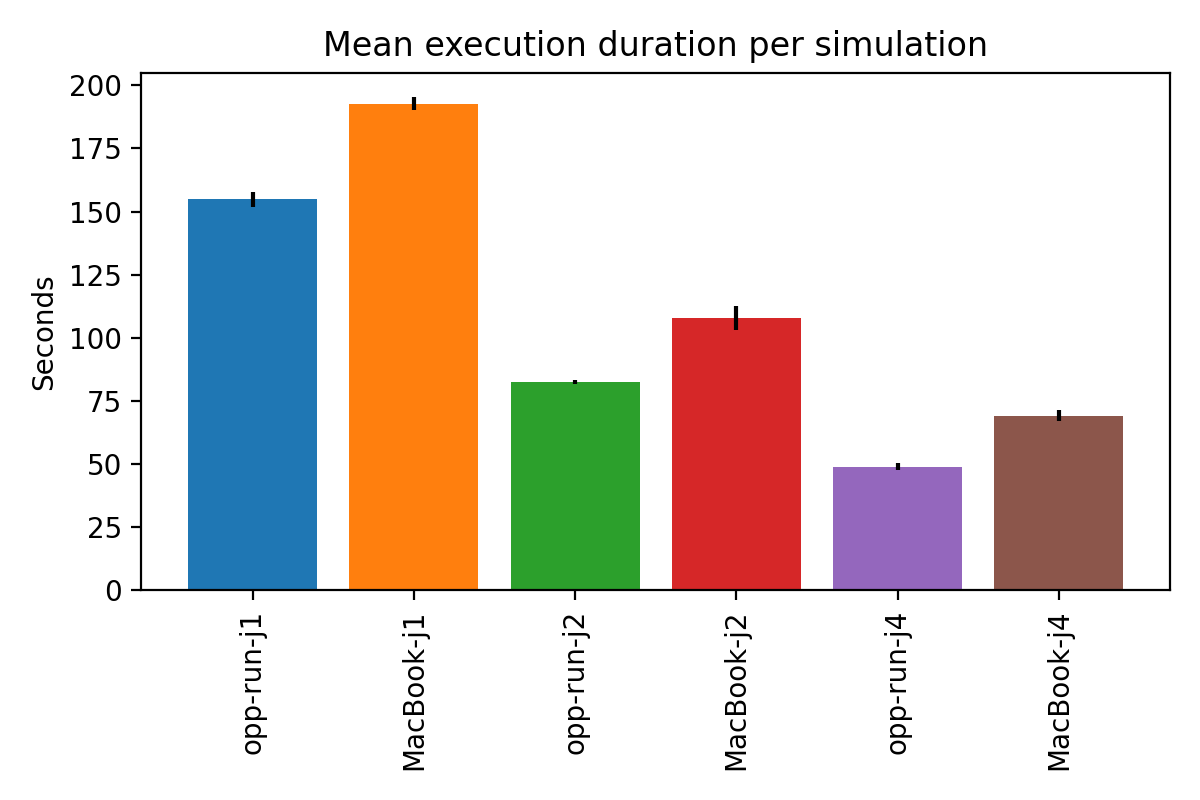
\includegraphics[width=250pt]{images/eval/overhead/Mean execution duration per simulation}
  \caption{Overhead: Mean execution duration per simulation}
  \label{fig:eval-overhead}
\end{figure}

Figure ~\ref{fig:eval-overhead-run} shows the average execution time per simulation-run. Scenario “MacBook-j4” has a slightly slower execution time because it is subject to thermal throttling effects. 

\begin{figure}[h]
  \centering
  \includesvg[width=250pt]{images/eval/overhead/Mean execution duration per simulation-run.svg}
  \caption{Overhead: Mean execution duration per simulation run}
  \label{fig:eval-overhead-run}
\end{figure}





\section{Connection overhead}

Providers and consumers connect over three ways: over a TCP connection in the local network, over a peer-to-peer UDP connection or over a TCP connection over a relay server. These connections can have different transfer rates which influence how fast simulation results can be transferred between the consumer and providers. Slow transfer rates are a bottleneck.

The local connection should be fastest, because the traffic doesn't leave the local network. The peer-to-peer connection should be second because it leaves the local network but is sent to the peer directly. The slowest should be the relay connection because the traffic is relayed by a central point. Figure \ref{fig:eval-connect-transfer} shows the download and upload transfer rates. The difference between the peer-to-peer and relay rates are neglectable, but it should be noted that at the time of the experiment no other client used the relay connection at the server. The peer-to-peer connection is preferred because it reduces traffic at the broker and is less susceptible.

\begin{figure}[h]
  \centering
  \includesvg[width=250pt]{images/eval/connect/Transfer Rate.svg}
  \caption{Connect: Transfer rates for the three connection ways}
  \label{fig:eval-connect-transfer}
\end{figure}

\section{Docker overhead}

For convenience and security reasons the provider software can be started from a Docker container. The Docker virtualization adds some overhead that can be seen in Figure \ref{fig:eval-docker-sim-run}. The measured overhead is approximately 15\%.

\begin{figure}[h]
  \centering
  %\includesvg[width=250pt]{images/eval/docker/Mean execution duration per simulation.svg}
  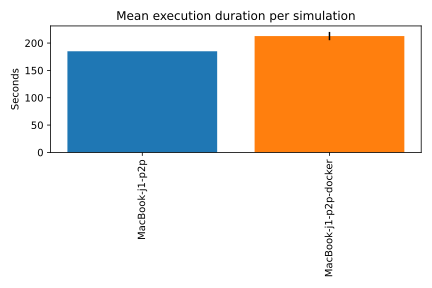
\includegraphics[width=250pt]{images/eval/docker/Mean execution duration per simulation}
  \caption{Docker: Mean execution duration per simulation}
  \label{fig:eval-docker-sim-run}
\end{figure}




\section{Maximal Parallelization}

The Figure \ref{fig:eval-aws-duration} shows the effect of nearly complete parallelization. The “tictoc” simulation example has a total of 78 simulation-runs. The scenario “AWS-j64” has a total of 64 CPUs that can start 64 simulation-runs in parallel. The data shows that a simulation which is executed with one CPU core needs a total of 184 seconds. A simulation that is executed with 64 CPU cores just needs 18 seconds, which is a speed up of approximately 10 times.

\begin{figure}[h]
  \centering
  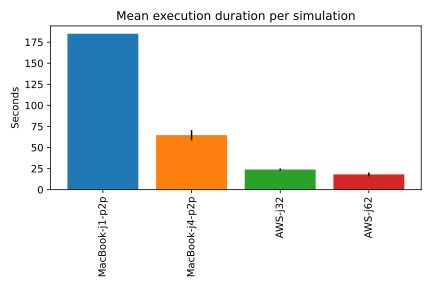
\includegraphics[width=250pt]{images/eval/aws/Mean execution duration per simulation}
  \caption{AWS: Mean execution duration per simulation}
  \label{fig:eval-aws-duration}
\end{figure}

Figure \ref{fig:eval-aws-transfer} shows that the download and upload transfer rates are approximately the same.

\begin{figure}[h]
  \centering
  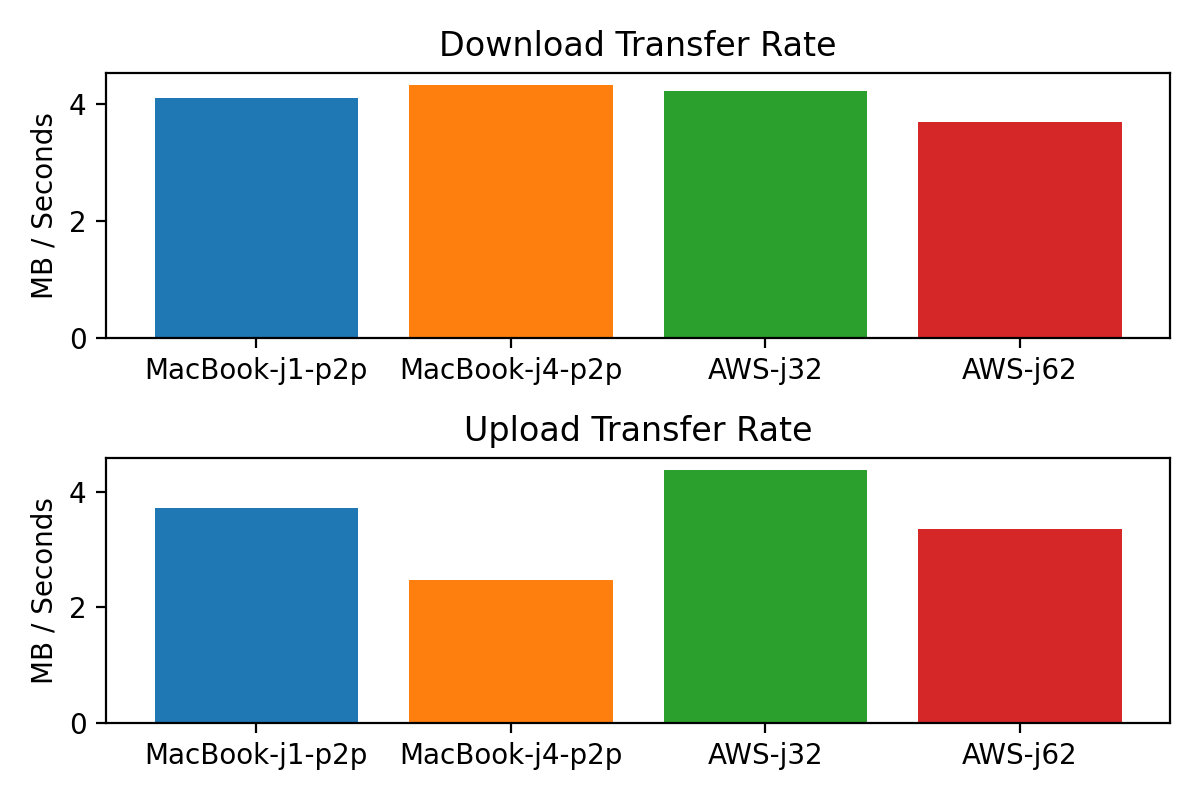
\includegraphics[width=250pt]{images/eval/aws/Transfer Rate}
  \caption{AWS: Transfer rates for the scenarios}
  \label{fig:eval-aws-transfer}
\end{figure}

	\chapter{Conclusion}

This work demonstrates the requirements and conditions for fast and reliable scheduling of discrete-event simulation runs in a heterogeneous edge computing environment.

Simulations can be intense computational tasks. Researchers often need to procure cloud resources to run simulations in an acceptable duration. Cloud resources can be costly to operate and involve bureaucratic hurdles. The spontaneous and cost-efficient involvement of idle resources like old laptops or Raspberry Pis is with related programs not possible. The distribution of simulations to many end-user devices is an attractive way to improve simulation run times without producing huge bills. 

OMNeT++ is a discrete event simulation framework. Simulations written with OMNeT ++ can be distributed relatively easily because they consist of smaller simulation runs that can be operated independently and in parallel.

Related efforts that distribute and parallelize simulations written with OMNeT++ are mostly deprecated and lack the ability to add resource providers on the fly and in separate networks. The efforts are not embedded into a peer-to-peer network like the tool developed by this thesis.

This thesis developed a novel approach for distributing OMNeT++ simulations using Go, gRPC, Docker, and UDP-Holepunching techniques. 
Resource consumers and providers try to communicate directly to reduce traffic over a central point. Providers have a robust allocation process in place to assign means to consumers. The provider executables are bundled with an OMNeT++ environment into a Docker image to ensure a safe and convenient deployment method. The simulation results are downloaded and extracted to the source directory like they were run locally.

In real-world trials, the execution time for the simulations was reduced significantly by employing multiple devices. The effect of nearly complete parallelization is quite impressive. It proves that processing a simulation in a distributed application makes much sense despite some overhead expenses. For example, it shows that a simulation that executes with 64 CPUs is about ten times faster than a process with only one CPU. 

The technical foundation of peer-to-peer communication over gRPC between providers and consumers can also be applied to other tasks. A remote SDK could be developed to execute generic code on providers, which extends possibilities significantly for many areas beyond simulations. A batch queuing system for generic tasks could be developed relatively quickly because most concepts for delivery and transport are already in place.

The optimization of bottle negs like uploading and downloading files had beneficial effects for the user experience. An effort worth looking at is the evolution of the linear storage package to a full-scale bit-torrent like a distributed storage system that circumvents upload and download thresholds. A second approach is the central storage of files on high bandwidth machines.

Another appealing research area is the research in building a "social network" for sharing resources. It would be interesting to understand under which circumstances people are inclined to share resources with others. One research question could be how much consumers are inclined to pay and how much reward providers expect for their services. A bidding system may be interesting to contemplate. In conjunction with this, another riveting area of research is the exploration of intelligent scheduling on algorithms on the provider and consumers' side. But also other incentives than money offer opportunities, like the devotion of resources to sciences in user-aligned concerns.

	\cleardoublepage
	
	% bibliography
	\frontmatter
	%\nocite{wiki:wissarbeit}
	\bibliographystyle{alphadin}
	\bibliography{references}
	\cleardoublepage

	% affidavit
		\chapter*{Eidesstattliche Versicherung}
\renewcommand*\chapterpagestyle{empty}
\addcontentsline{toc}{chapter}{Eidesstattliche Versicherung}
Hiermit versichere ich an Eides statt, dass ich die vorliegende Arbeit im Studiengang B.Sc. Informatik
selbstständig verfasst und keine anderen als die angegebenen Hilfsmittel – insbesondere keine im Quellenverzeichnis nicht benannten Internet-Quellen – benutzt habe.
Alle Stellen, die wörtlich oder sinngemäß aus Veröffentlichungen entnommen wurden, sind als solche kenntlich gemacht. 
Ich versichere weiterhin, dass ich die Arbeit vorher nicht in einem anderen Prüfungsverfahren eingereicht habe und die eingereichte schriftliche Fassung der auf dem elektronischen Speichermedium entspricht.
\vspace{1cm} 

\noindent Hamburg, den \uline{~~~~~~~~~~~~~~~~~~~~~~~~~~~~~~~}~~~~~~~Unterschrift: \uline{~~~~~~~~~~~~~~~~~~~~~~~~~~~~~~~~~~~~~~~~~~~~~~~~~~} 

\let \cleardoublepage \clearpage

\noindent\begin{minipage}{\textwidth}
	
\vspace{1cm} 
\chapter*{Veröffentlichung}
Ich stimme der Einstellung der Arbeit in die Bibliothek des Fachbereichs Informatik \\zu.
\vspace{1cm}\\ 
\noindent Hamburg, den \uline{~~~~~~~~~~~~~~~~~~~~~~~~~~~~~~~}~~~~~~~Unterschrift: \uline{~~~~~~~~~~~~~~~~~~~~~~~~~~~~~~~~~~~~~~~~~~~~~~~~~~}
\end{minipage}

	
\end{document}